\section{Method}
In this section, the tools and the implemented system are specified. 

\subsection{Peripherals}

The external hardware required for developing the project will be described in detail.

\subsubsection{Tobii Pro Nano Eye Tracker}

\begin{figure}[ht]
    \centering
    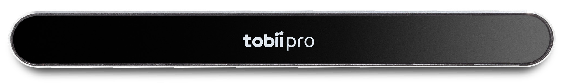
\includegraphics[width=0.7\textwidth]{images/tobii-pro-nano.png}
    \caption{Tobii Pro Nano Eye Tracker. Source: \citep{manual:tobiipronano}}
    \label{fig:tobii-eye-tracker}
\end{figure}

The Tobii Pro Nano Eye Tracker, shown in figure \ref{fig:tobii-eye-tracker}, uses a corneal reflection, dark and bright pupil combination, one-camera system. It supports screen sizes up to 19 inches, introduces a 17 ms system latency. \citep{manual:tobiipronano}

It is characterized by its lightweight and compact form; which makes it easy to carry, and ultimately enabled an easier usability testing process. On the other hand, Tobii Eye Trackers are compatible with the \verb|tobii-research| SDK for python, which allows for controlling the device without the need for a graphical user interface.

This device prompted the idea for the project.

\subsubsection{Microphone}

The microphone serves as a mediator of interaction, enabling the capture of verbal cues essential for the analysis of words that then get turned into commands thanks to the natural language processing. It also serves as an way of qualitative data acquisition, for recording each participant response for usability testing.

\subsection{System Design}

Given the system requirements and all of the peripherals it has to handle, a software architecture design was needed, in order to satisfy all the functional and non-functional requirements.

\subsubsection{Software Architecture}

\begin{figure}[ht]
    \centering
    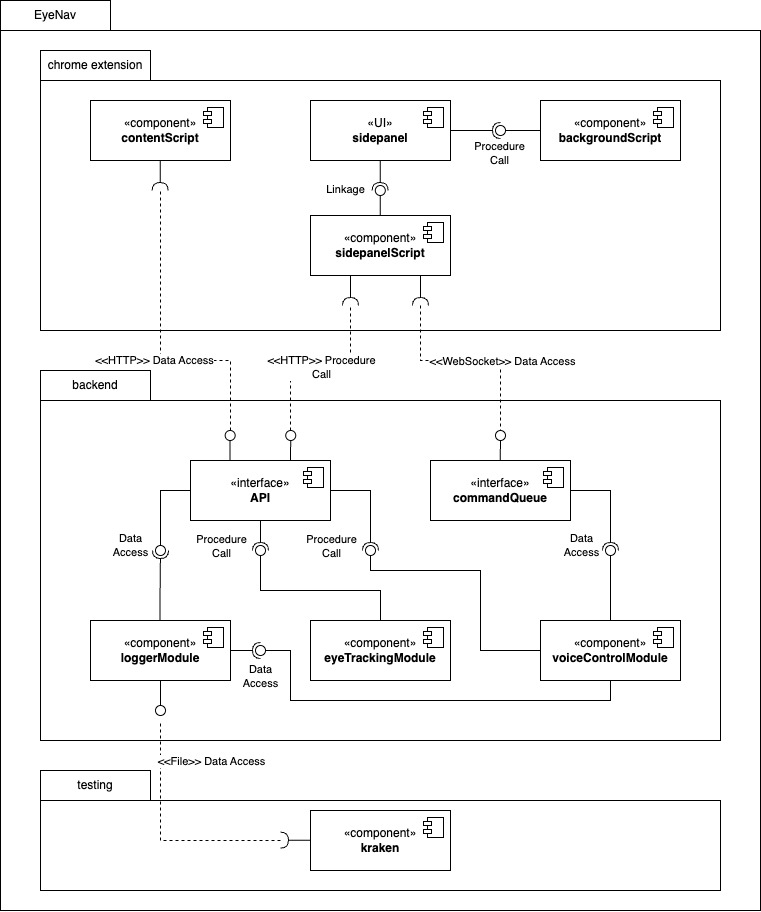
\includegraphics[width=0.85\textwidth]{images/components-diagram.jpg}
    \caption{Architecture described in components}
    \label{fig:components-diagram}
\end{figure}

The software components are shown in figure \ref{fig:components-diagram}. The important takeaway here is the understanding of which component communicates with each other, and how this comunication is happening (protocol, procedure, etc) and in which environment. This also showcases how the architecture of the system works in a fullstack-like matter, where the frontend (chrome extension) communicates with the backend, and the additional testing module. 

\begin{figure}[ht]
    \centering
    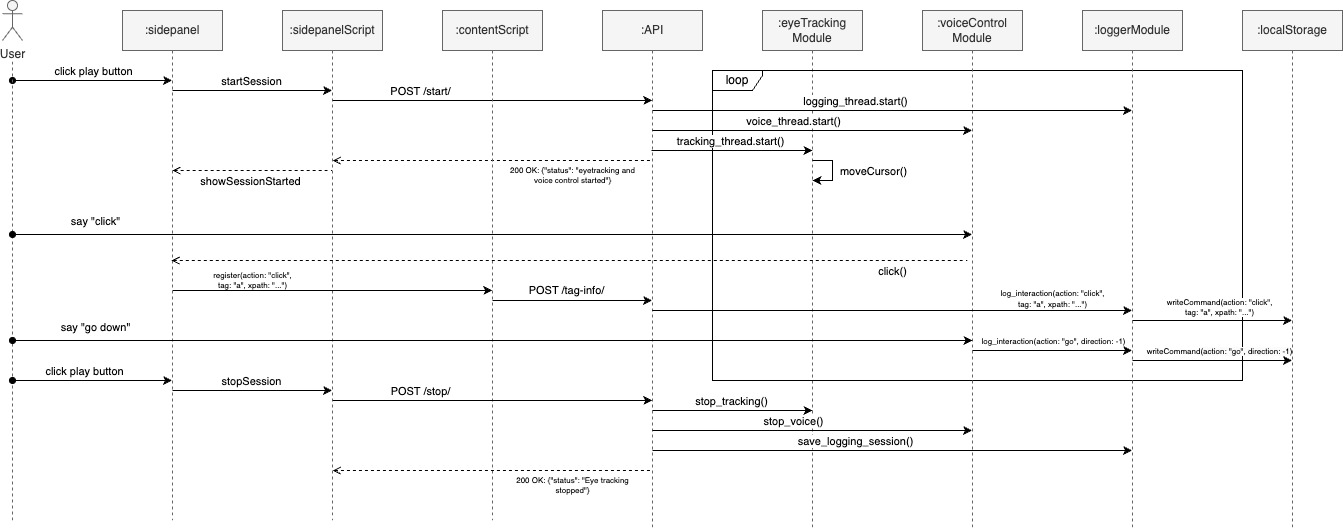
\includegraphics[width=0.85\textwidth]{images/sequence-diagram.jpg}
    \caption{An user clicking and scrolling sequence}
    \label{fig:sequence-diagram}
\end{figure}

Figure \ref{fig:sequence-diagram} displays a sequence diagram where a user starts a simple session, in which they click an element on screen and scroll down. The purpose of this illustration is to showcase how the system behaves and which component, from the previous component diagram, is responsible for handling each instructions. 

This system works through the power of multithreading and concurrency, therefore, showcasing when each process is being called and by who helps to illustrate the functionality better.



\subsection{Implementation}
A prototype for this idea was developed, which lets the user control the web browser using their gaze visualization and voice for command instructions. The prototype is started using the frontend, and the backend needs to be running prior to said initialization. 

All of the source code for this project is hosted in a GitHub repository.\footnote{\url{https://github.com/juanyepesp/EyeNav}} The repository holds the code for this documentation, the backend module, the chrome extension and the testing module.

\subsubsection{Chrome Extension}
In Chrome versions 114 and later, it is possible to develop a sidepanel, which effectively gives the ability to create a secondary and completely independent webpage (or at least from the primary webpage) that is always visible to the user. This is an awesome capability since it allows for the system to display important information relevant to the user. For instance, the voice command that the voice recognition module detected, or the different commands that can be used and how, etc.

Developing a chrome extension, or at least one with a sidepanel, is effectively the same as doing a webpage. The only extra step to creating one is to use a \verb|manifest.json| that tells the browser the code will be packaged into an extension. The rest is plain javascript for functionality, HTML for structure and CSS for styles. 

There are also some tricky parts that needed to be adressed. Since the system needs to register which HTML tag the user clicks in a given moment, the extension needs to handle each click using an event listener. However, this needs to be implemented carefully for dynamically created elements, since adding an event listener on top can eliminate certain functionalities of the webpage.

\subsubsection{Backend}

The backend needed to include several components in order to achieve all of the functional requirements. Following the diagram detailed in figure \ref{fig:components-diagram}, here the implementation of each one will be described.

As a disclaimer, every part of this system is running locally on a single computer, ensuring data privacy, minimal latency and overall a strong performance.

\begin{itemize}
    \item \verb|API|
    
    Implemented in the \verb|main.py| file, this component is the primary way of talking with the backend and exposes the messages necessary for starting and stopping a session, and registering each click tag. 
    
    \item \verb|commandQueue|
    
    The command queue, is the tunnel of information for each voice command that the voice control module recognizes. It uses websockets instead of HTTP for ensuring a fast and streamlined command display; ensuring minimal latency perceived by the user in the chrome extension. 

    \item \verb|loggerModule|
    
    Similarly, this module also uses a queue for handling instruction writing on the testing files, called features. Each feature is created once the session is started, and needs to be handled on a queue for impeding data races. 
    
    \item \verb|eyeTrackingModule|
    
    The eyetracking module uses the \verb|tobii-research| module part of the tobii pro sdk for Python. It enables for the programatic control of the eyetracker whilst smoothly moving the cursor to each new position it detects. 
    
    \item \verb|voiceControlModule|
    
    The voice control module was developed using \verb|Vosk|, an open sourced framework for loading language modules locally. \verb|Vosk| allows for downloading different models based on language. This module is also responsible for translating each correct voice command into an actual computer command, while adding to the queue said commands for the logging module to process.
    
\end{itemize}

\subsubsection{Testing}

The testing module is much more straightforward and concrete, primarily due to the Kraken module handling most of the responsibilities. The only necessary files that had to be created were the step definition file and each feature (those are the tests to be executed). The step definitions are written in Gherkin syntax and include each action the user took; they need to be defined for the webdriver to execute them. On the other hand, the features were created previously by the logger module.

